\documentclass[zihao=false,fontset=windows]{ctexart}
% ctexart 不接受任意 pt 选项。正文改 {10pt}，方括号里是行距。
\usepackage{scrextend}
\changefontsizes[12pt]{10pt}

\usepackage[a4paper,left=2.35cm,right=2.35cm,top=1.7cm,bottom=1.9cm]{geometry}
\usepackage{xcolor}
\usepackage{graphicx}
\usepackage{amsmath,amssymb}
\usepackage{enumitem}
\usepackage{needspace}
\usepackage{tabularx}
\usepackage{colortbl}
\usepackage{listings}
\usepackage{hyperref}
\usepackage[most]{tcolorbox}

\definecolor{feishuText}{RGB}{31,35,41}
\definecolor{feishuBlue}{RGB}{36,91,219}
\definecolor{feishuRed}{RGB}{216,57,49}
\definecolor{feishuGray}{RGB}{100,106,115}
\definecolor{feishuGray2}{RGB}{143,149,158}
\definecolor{feishuPinkBg}{RGB}{251,191,188}
\definecolor{quoteBar}{RGB}{51,112,255}
\definecolor{codebg}{RGB}{245,246,247}
\definecolor{codeborder}{RGB}{222,224,227}
\definecolor{inlinebg}{RGB}{242,243,245}
\definecolor{callRed}{RGB}{253,226,226}
\definecolor{callOrange}{RGB}{255,245,235}
\definecolor{callYellow}{RGB}{254,255,240}
\definecolor{callGreen}{RGB}{240,251,239}
\definecolor{callBlue}{RGB}{240,244,255}
\definecolor{callRedSoft}{RGB}{254,241,241}
\definecolor{callSun}{RGB}{255,255,204}
\definecolor{tableHead}{RGB}{242,243,245}
\definecolor{tableRule}{RGB}{222,224,227}
\definecolor{codeText}{RGB}{31,35,41}
\definecolor{codeKeyword}{RGB}{0,0,255}
\definecolor{codeComment}{RGB}{0,128,0}
\definecolor{codeString}{RGB}{163,21,21}

\setmainfont{Times New Roman}
\setCJKmainfont{Microsoft YaHei}[AutoFakeBold=2.2]
\setCJKsansfont{Microsoft YaHei}[AutoFakeBold=2.2]
\setCJKmonofont{Microsoft YaHei}[AutoFakeBold=2.2]
\setmonofont{Consolas}
\newfontfamily\emojifont{Segoe UI Emoji}

\hypersetup{
  colorlinks=true,
  urlcolor=feishuBlue,
  linkcolor=feishuBlue,
  unicode=true,
  pdftitle={Qwen-VL}
}

\setlength{\parindent}{0pt}
\setlength{\parskip}{0.42em}
\setlength{\fboxsep}{1.5pt}
\setlength{\emergencystretch}{3em}
\linespread{1.28}
\color{feishuText}
\arrayrulecolor{tableRule}
\urlstyle{same}

\setlist[enumerate]{label=\textcolor{feishuBlue}{\arabic*.}, leftmargin=1.7em, itemsep=0.22em, topsep=0.28em, parsep=0.08em, partopsep=0pt}
\setlist[itemize,1]{label=\textcolor{feishuBlue}{\textbullet}, leftmargin=1.35em, itemsep=0.18em, topsep=0.25em, parsep=0.06em, partopsep=0pt}
\setlist[itemize,2]{label=\textcolor{feishuBlue}{◦}, leftmargin=1.45em, itemsep=0.12em, topsep=0.15em}
\setlist[itemize,3]{label=\textcolor{feishuBlue}{\rule[0.18em]{0.38em}{0.38em}}, leftmargin=1.55em, itemsep=0.1em, topsep=0.12em}

\newcommand{\feiEmoji}[1]{{\emojifont #1}}
\newcommand{\incode}[1]{\colorbox{inlinebg}{\ttfamily\small #1}}
\newcommand{\bigmath}[1]{%
  \begin{center}\large$\displaystyle #1$\end{center}%
}

\lstset{
  language=Python,
  basicstyle=\ttfamily\footnotesize\color{codeText},
  keywordstyle=\color{codeKeyword},
  commentstyle=\color{codeComment},
  stringstyle=\color{codeString},
  showstringspaces=false,
  breaklines=true,
  columns=fullflexible,
  keepspaces=true,
  tabsize=4,
  upquote=true,
  aboveskip=2pt,
  belowskip=0pt,
  xleftmargin=0pt,
  frame=none
}

\tcbset{
  feishubase/.style 2 args={
    enhanced,
    boxrule=0pt,
    arc=8pt,
    left=10pt,
    right=10pt,
    top=7pt,
    bottom=7pt,
    before skip=6pt,
    after skip=6pt,
    colback=#1,
    colframe=#1,
    before upper={\feiEmoji{#2}\hspace{0.45em}\ignorespaces}
  }
}
\newtcolorbox{feishubox}[2]{feishubase={#1}{#2}, breakable}
\newtcolorbox{feishuboxnb}[2]{feishubase={#1}{#2}}

\newtcolorbox{feishuquote}{
  enhanced,
  breakable,
  boxrule=0pt,
  leftrule=3pt,
  arc=0pt,
  colframe=quoteBar,
  colback=white,
  left=8pt,
  right=2pt,
  top=2pt,
  bottom=2pt,
  before skip=4pt,
  after skip=4pt,
  before upper=\color{feishuGray}
}

\newtcolorbox{feishucode}{
  enhanced,
  breakable,
  colback=codebg,
  colframe=codeborder,
  boxrule=0.6pt,
  arc=6pt,
  left=6pt,
  right=6pt,
  top=5pt,
  bottom=4pt,
  before skip=6pt,
  after skip=6pt
}


\begin{document}
{\zihao{1}\bfseries Qwen-VL\par}
{\small\color{feishuGray} 来源：\href{https://scnajei2ds6y.feishu.cn/wiki/YDpewbRHwiLNAikDH1HcUtNInve}{飞书原文}；2025年9月27日修改\par}

\par\vspace{0.95em}\noindent{\zihao{-2}\bfseries \textcolor{feishuBlue}{1.} 模型架构}\par\vspace{0.28em}

\begin{tcbraster}[raster columns=2,raster column skip=9pt,raster equal height=rows]
\begin{tcolorbox}[blankest]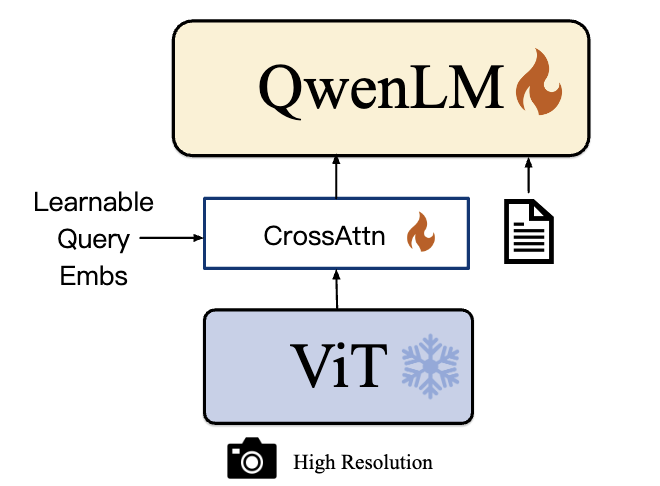
\includegraphics[width=\linewidth]{images/Qwen-VL/fig-01.png}\end{tcolorbox}
\begin{tcolorbox}[blankest]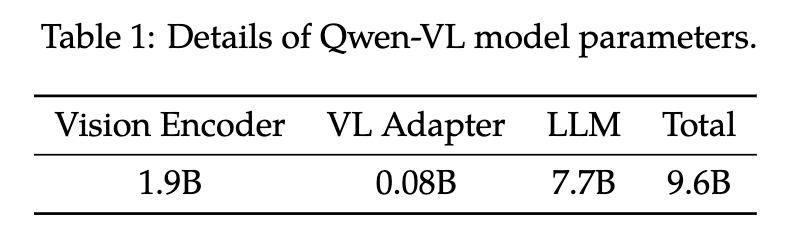
\includegraphics[width=\linewidth]{images/Qwen-VL/fig-02.png}\end{tcolorbox}
\end{tcbraster}

\par\vspace{0.95em}\noindent{\zihao{3}\bfseries \textcolor{feishuBlue}{1.1} ViT}\par\vspace{0.28em}

视觉编码器的架构和预训练权重来自于Openclip的ViT-bigG模型。ViT-bigG/14训练使用LAION-2B（采样自\href{https://laion.ai/blog/laion-5b/}{LAION-5B}的英文标注图文pair数据，框架是\href{https://github.com/mlfoundations/open_clip}{OpenCLIP}。\par

在训练和推理过程中，将输入图像调整到特定的分辨率，然后通过将图像分割成大小为14的图块来处理它们，生成图像特征。\par

\par\vspace{0.95em}\noindent{\zihao{3}\bfseries \textcolor{feishuBlue}{1.2} Position-aware Vision-Language Adapter}\par\vspace{0.28em}

1）为了缓解由于长图像特征序列而产生的效率问题，Qwen-VL引入了一个视觉-语言适配器，用于压缩图像特征。适配器包括一个随机初始化的单层交叉注意力模块（single-layer cross-attention module initialized randomly）。此模块使用一组可训练的向量（嵌入）作为query，使用来自视觉编码器的图像特征作为交叉注意力操作的keys、values。这个机制将视觉特征序列压缩到固定长度的256。\par

注意，这个模块和\href{https://scnajei2ds6y.feishu.cn/wiki/SEDGwBr2TimSUpkTkOlclwfSn5f}{mPLUG-OWL(2023, Alibaba)}的区别在于这里并没有把Q拼接在KV上\par

2）\textbf{为了缓解1D位置编码对图片空间位置造成的损失，使用2D绝对位置编码。}\par

这里是有2个位置编码：\par

\begin{itemize}

\item VIT有自己的可以学习的1d-PE

\item Resample有自己的不可以学习的2d-PE

\end{itemize}

\par\vspace{0.95em}\noindent{\zihao{3}\bfseries \textcolor{feishuBlue}{1.3} LLM}\par\vspace{0.28em}

Qwen-VL的大型语言模型使用了来自Qwen-7B模型的\textbf{预训练}权重。\par

\Needspace{9cm}
\par\vspace{0.95em}\noindent{\zihao{-2}\bfseries \textcolor{feishuBlue}{2.} 训练}\par\vspace{0.28em}

\begin{center}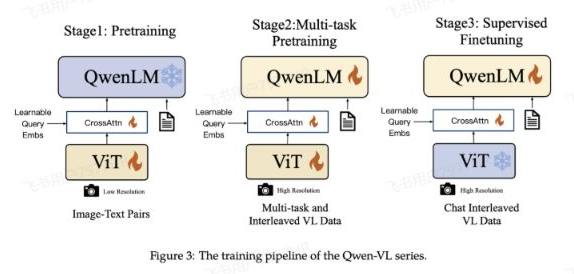
\includegraphics[width=0.98\textwidth]{images/Qwen-VL/fig-03.png}\end{center}

三阶段训练：\par

\begin{itemize}

\item Stage1 为预训练，目标是使用大量的图文Pair对数据对齐视觉模块和LLM的特征，这个阶段冻结LLM模块的参数；

\item Stage2 为多任务预训练，使用更高质量的图文多任务数据（主要来源于开源VL任务，部分自建数据集），更高的图片像素输入，全参数训练；

\item Stage3 为指令微调阶段，这个阶段冻结视觉Encoder模块，使用的数据主要来自大模型Self-Instruction方式自动生成，目标是提升模型的指令遵循和多轮对话能力。

\end{itemize}

\par\vspace{0.95em}\noindent{\zihao{3}\bfseries \textcolor{feishuBlue}{2.1} Stage 1}\par\vspace{0.28em}

损失函数仍然是针对文本标记的训练目标是最小化文本标记的交叉熵（cross-entropy）。\par

\begin{itemize}

\item 超参数设置

\end{itemize}

{\color{feishuGray} 1）AdamW优化器，并设置了以下超参数：$\beta_1$ = 0.9、$\beta_2$ = 0.98、$\varepsilon$= 1e−6\par}

{\color{feishuGray} 2）余弦学习率调度（cosine learning rate schedule）。最大学习率（maximum learning rate）为2e−4，最小学习率（minimum learning rate）为1e−6，线性热身（linear warm-up）步数为500步。\par}

{\color{feishuGray} 3）使用了权重衰减（weight decay）为5e−2和梯度剪切（gradient clipping）为1.0来优化模型的训练过程。\par}

{\color{feishuGray} 4）训练为5w步。\par}

\begin{itemize}

\item 数据来源

\end{itemize}

\begin{center}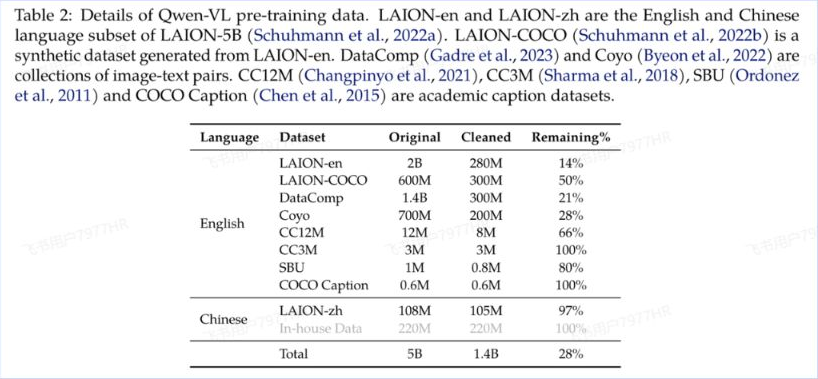
\includegraphics[width=0.98\textwidth]{images/Qwen-VL/fig-04.png}\end{center}

{\color{feishuGray} Qwen-VL模型的第一个预训练阶段使用了一个大规模、弱标记的、通过网络爬取得到的图像文本对数据集。原始数据集中包含了50亿对图像文本对，而剩余的数据经过处理后仍然有14亿对，其中\textcolor{feishuRed}{77.3\%为英文文本，22.7\%为中文文本}。\par}

\textbf{总计14亿对样本，5000亿的图像文本tokens。}\par

\par\vspace{0.95em}\noindent{\zihao{3}\bfseries \textcolor{feishuBlue}{2.2} Stage 2}\par\vspace{0.28em}

Qwen-VL模型采用了高质量和细粒度的视觉-语言（VL）标注数据\par

采用了更大的输入分辨率和交错的图像-文本数据。\par

具体来说，Qwen-VL模型在第二个预训练阶段同时进行了以下七个任务的训练：\par

\begin{itemize}

\item 图像描述（Captioning）

\item 视觉问答（VQA）

\item 定位任务（Grounding）

\item 参考定位和定位描述的双重任务（Ref Grounding 和 Grounded Cap.）

\item 光学字符识别（OCR）

\item 文本生成（Text Generation）

\end{itemize}

在这个阶段，作者综合利用了不同的数据源和任务，使得模型能够在多方面进行训练，从而提升其对于图像与文本的综合理解能力。\par

\Needspace{11cm}
\par\vspace{0.95em}\noindent{\zihao{3}\bfseries \textcolor{feishuBlue}{2.3} Stage 3}\par\vspace{0.28em}

在监督微调阶段，Qwen-VL模型通过引入额外的指导微调数据来提升其交互和对话能力，从而生成了交互式的Qwen-VL-Chat模型。这些多模态的指导调整数据主要来自于图像描述或对话数据，这些数据可以通过LLM self-instruction生成。然而，这些数据通常只涵盖了单一图像对话和推理，且仅限于对图像内容的理解。因此，作者们通过手动标注、模型生成和策略串联等方法构建了一组额外的对话数据，以将定位和多图像理解能力融入到Qwen-VL模型中。\par

这样做的目的是确保模型可以有效地将这些能力传递到更广泛的语言和问题类型中，从而提升了模型在交互和对话方面的性能。在这个阶段，作者们将模型的视觉编码器冻结，仅优化语言模型和适配器模块，以保证模型的训练稳定和有效。\par

训练Qwen-VL-Chat模型的微调参数设定：\par

\begin{itemize}

\item 全局批次大小为128的训练方式

\item 使用了具有最大学习率1e-5、最小学习率1e-6和线性预热3000步的学习率调度。

\end{itemize}

微调模版：\par

\begin{center}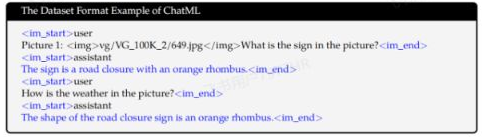
\includegraphics[width=0.98\textwidth]{images/Qwen-VL/fig-05.png}\end{center}
\end{document}
